\subsection{Visualizzazione dataset caricato}

\begin{figure}[H]
    \centering
    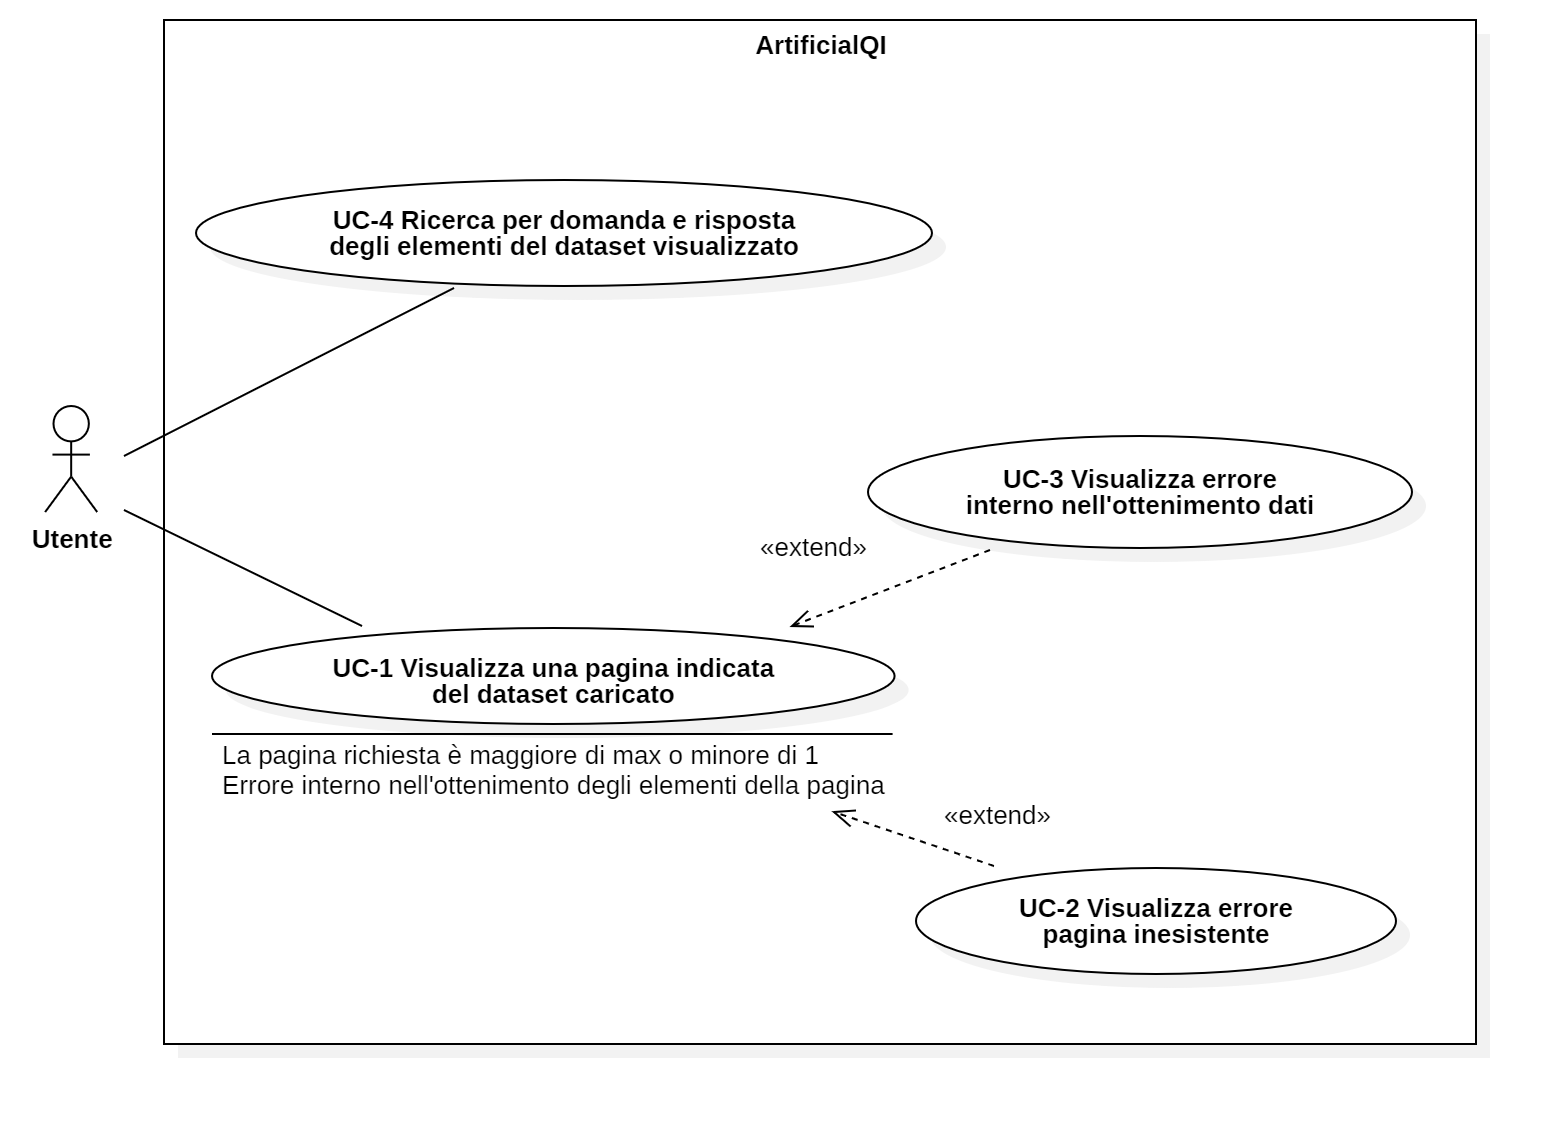
\includegraphics[scale=0.23]{Sezioni/UseCase/Immagini/VisualizzazioneDatasetCaricato}
    \caption{Diagramma visualizzazione dataset caricato.}
\end{figure}

\begin{usecase}{UC-1}{Visualizza il contenuto del dataset caricato}
    \label{uc:UC-1}    
    
    \req{\hyperref[ru:RUO-1]{RUO-1}} 

    \pre{
        \item L'utente ha caricato un dataset
    }

    \post{
        \item Viene visualizzata la prima pagina del dataset caricato
    }
    
    \actor{Utente}

    \subactors{}

    \trigger{L'utente vuole visualizzare il contenuto del dataset caricato}
    
    \inc{\hyperref[uc:UC-2]{UC-2}}

    \base{}

    \scenario{
        \item L'utente richiede la visualizzazione del contenuto del dataset caricato
        \item Viene visualizzata la prima pagina del dataset caricato o l'ultima pagina richiesta dall'utente secondo \hyperref[uc:UC-2]{UC-2}
    }

    \subscenario{
        \item[1.1] I'ultima versione del dataset caricato è vuoto:
        \begin{itemize}
            \item[a.] Viene indicato all'utente che il datataset caricato è vuoto
        \end{itemize}
    }
\end{usecase}


\begin{usecase}{UC-2}{Visualizza pagina dataset caricato}
    \label{uc:UC-2}
    
    \req{} 

    \pre{
        \item La pagina del dataset caricato da visualizzare esiste
    }

    \post{
        \item Viene visualizzato il contenuto della pagina del dataset caricato
    }
    
    \actor{Utente}

    \subactors{}

    \trigger{Il sistema deve visualizzare una pagina del dataset caricato}

    \inc{}

    \base{}

    
    \scenario{
        \item Il sistema ottiene gli elementi che compongono la pagina del dataset caricato
        \item Gli elementi vengono visualizzati in una lista
    }

    \subscenario{
        \item[1.1] Errore interno durante l'ottenimento degli elementi:
        \begin{itemize}
            \item[a.] \hyperref[uc:UC-3]{UC-3}
        \end{itemize}
    }

\end{usecase}

\begin{usecase}{UC-3}{Visualizza errore interno nell'ottenimento dati}
    \label{uc:UC-3}
    
    \req{} 

    \pre{
        \item Avviene un errore interno al sistema durante l'ottenimento di uno o più dati gestiti da esso    
    }

    \post{
        \item L'utente è a conoscenza dell'errore interno avvenuto
    }

    \actor{Utente}

    \subactors{}

    \trigger{Il sistema riscontra un errore interno durante l'ottenimento di dati}

    \inc{}

    \base{}

    \scenario{
        \item Viene mostrato un messaggio di errore che informa l'utente sulla natura dell'errore
    }

    \subscenario{}

\end{usecase}


\begin{usecase}{UC-4}{Cambia pagina del dataset visualizzato}
    \label{uc:UC-4}
    
    \req{\hyperref[ru:RUO-1]{RUO-1}} 

    \pre{
        \item L'utente sta visualizzando il dataset caricato \hyperref[uc:UC-1]{UC-1}
        \item Il dataset caricato non è vuoto
    }

    \post{
        \item L'utente visualizza la pagina del dataset caricato che ha richiesto
    }
    
    \actor{Utente}

    \subactors{}

    \trigger{L'utente vuole visualizzare una pagina del dataset caricato}
    
    \inc{\hyperref[uc:UC-2]{UC-2}}

    \base{}

    \scenario{
        \item L'utente richiede la visualizzazione di una precisa pagina del dataset caricato
        \item Il sistema controlla che la pagina richiesta esista
        \item Viene visualizzata la pagina richiesta secondo \hyperref[uc:UC-2]{UC-2} 
    }

    \subscenario{
        \item[2.1] La pagina richiesta non esiste ovvero è minore di uno o maggiore della pagina massima:
        \begin{itemize}
            \item[a.] \hyperref[uc:UC-5]{UC-5}
        \end{itemize}
    }

\end{usecase}

\begin{usecase}{UC-5}{Visualizza errore pagina inesistente}
    \label{uc:UC-5}
    
    \req{} 

    \pre{
        \item Il controllo di validità del numero di pagina fallisce
    }

    \post{
        \item L'utente capisce che la pagina richiesta non esiste e conosce il range di pagine valide
    }

    \actor{Utente}

    \subactors{}

    \trigger{Il sistema ha ricevuto una richiesta di visualizzazione per una pagina inesistente}

    \inc{}

    \base{}

    \scenario{
        \item Viene visualizzato un messaggio di errore che informa l'utente che la pagina richiesta non esiste
        \item Viene indicato il range di pagine valide 
    }

    \subscenario{}

\end{usecase}


\begin{usecase}{UC-6}{Ricerca per domanda e risposta degli elementi del dataset visualizzato}
    \label{uc:UC-6}
    
    \req{\hyperref[ru:RUO-2]{RUO-2}} 

    \pre{
        \item L'utente sta visualizzando il dataset caricato \hyperref[uc:UC-1]{UC-1}
    }

    \post{
        \item Il dataset caricato viene ristretto all'insieme di elementi risultanti dalla ricerca
        \item Il dataset caricato ristretto viene visualizzato
    }
    
    \actor{Utente}

    \subactors{}

    \trigger{L'utente vuole eseguire una ricerca per domanda e risposta sul dataset caricato}
    
    \inc{\hyperref[uc:UC-1]{UC-1}}

    \base{}

    \scenario{
        \item L'utente specifica le parole chiave da utilizzare nella ricerca
        \item Il sistema ricerca gli elementi che contengono le parole chiave nella propria domanda e/o risposta
        \item Il sistema restringe internamente il dataset caricato agli elementi risultanti dalla ricerca
        \item Viene visualizzato il dataset caricato ristretto secondo \hyperref[uc:UC-1]{UC-1}
    }

    \subscenario{}

\end{usecase}